\documentclass[a4paper,11pt]{article}

\usepackage{oikos}
%% Useful packages
\usepackage{amsmath}
\usepackage{graphicx}
\usepackage[colorlinks=true, allcolors=blue]{hyperref}
%% Add the following packages in the oikos.sty file
\usepackage{textcomp}
\usepackage{mfirstuc}

% To add comments (begin)
\usepackage[textwidth=4.5cm]{todonotes}
\usepackage{geometry}
\geometry{verbose,letterpaper,tmargin=2.5cm,bmargin=2.5cm,lmargin=2.5cm,rmargin=5.5cm}
\newcommand{\nico}[1]{\todo[backgroundcolor=red!25,bordercolor=red]{\small #1}}
\newcommand{\nicoin}[1]{\todo[inline,backgroundcolor=red!25,bordercolor=red]{\small #1}}
\newcommand{\Mark}[1]{\todo[backgroundcolor=green!25,bordercolor=green]{\small #1}}
\newcommand{\Markin}[1]{\todo[inline,backgroundcolor=green!25,bordercolor=green]{\small #1}}
\newcommand{\kris}[1]{\todo[backgroundcolor=blue!25,bordercolor=blue]{\small #1}}
\newcommand{\krisin}[1]{\todo[inline,backgroundcolor=blue!25,bordercolor=blue]{\small #1}}
% To add comments (end)

%% new commands
\newcommand{\species}[1]{(\xmakefirstuc{\emph{#1}})}

%% Information about the paper

\title{Assessing the timing of territoriality and rutting behaviour in
  roe deer from GPS data}

\author{Morellet Nicolas, Bonenfant Christophe, Miele Vincent,
  \ldots\\ \& Hewison A.J. Mark}
  

\affiliations{Nicolas Morellet and A.J. Mark Hewison, CEFS, Université de
Toulouse, INRA, Castanet-Tolosan, France - e-mail addresses: Nicolas.Morellet@inra.fr (Nicolas Morellet); Mark.Hewison@inra.fr (A.J. Mark Hewison) -- Christophe Bonenfant and Vincent Miele, Université de Lyon, Université Lyon 1, CNRS, UMR5558,
  Laboratoire de Biométrie et Biologie {\'E}volutive, Bâtiment
  G. Mendel, 43 boulevard du 11 novembre 1918, F-69622, Villeurbanne,
  France - e-mail addresses: christophe.bonenfant@univ-lyon1.fr
  (Christophe Bonenfant); miele.vincent@univ-lyon1.fr (Vincent Miele) 
}

\begin{document}
%% set on/off for double spacing
%\doublespacing
\maketitle

\newpage
\begin{abstract}
Nice abstract here
\end{abstract}

\newpage
\section*{Introduction}

Mating and reproduction affect many facets of an individual phenotype,
changing its appearance and shape or shaping its life history and
behaviour \citep{Darwin1871}. Across species the mating system is
associated with a set of behaviours aiming at pairing individuals with
sexual partners and increasing their reproductive success
\citep{Emlen1977,Clutton-Brock1989a,Wittenberger1979}. Males of
polygynous species frequently engaged into intense male-male fights,
do not provide parental care to offspring and are often larger in size
than females. In monogamous species, parents of the two sexes do care
for the offspring \nico {Paternal care is often considered
synonymous with social monogamy, although it occurs in only
59\% of socially monogamous species (Lukas & Clutton-Brock,
2013 Lukas, D. & Clutton-Brock, T.H. (2013). The evolution of social
monogamy in mammals. Science 341,526–530.)}, females chose their mating partner carefully and males often show display courtship behaviour (Boogert, Fawcett & Lefebvre 2011) \nico{Boogert, N.J., Fawcett, T.W., Lefebvre, L., 2011. Mate choice for cognitive traits: a review of the evidence in nonhuman vertebrates. Behavioral Ecology 22, 447–459. https://doi.org/10.1093/beheco/arq173}. Mating behaviour
may also vary among populations or individuals of the same species
\citep{Lott1991,Dunbar1982}. The environmental context such as
population density or resource distribution can modulate what mating
behaviour is expressed by most males (Verner and Willson 1966; Caranza
et al. 1990). At the individual level, age, social status, body size
or physiological states are tightly linked with the decision to
reproduce and the type of mating tactic to be adopted. Being closely
associated to reproductive success and fitness, mating and
reproductive behaviours are under strong selection pressures and have
received a lot of attention from ecologists. A careful understanding
of the evolution of reproductive tactics and of mating systems hence
requires to assess if, when, where and how long an individual did
display reproductive-related behaviours.

Many species may, however, be secretive, inhabiting environments with
poor visibility or present a nocturnal activity, so that
reproductive-related behaviours are difficult to observe directly or
to quantify accurately \citep{maher_definitions_1995}. For instance,
we currently have a huge gap of knowledge in the reproductive
behaviour in the wild of most small felids (Mellen 1993)\nico{Mellen, J.D., 1993. A Comparative Analysis of Scent-Marking, Social and Reproductive Behavior in 20 Species of Small Cats ( Felis ). American Zoologist 33, 151–166. https://doi.org/10.1093/icb/33.2.151
}, as for example the jaguar \species{Panthera onca} (Leuchtenberger et al. 2009) \nico{Leuchtenberger, C., Crawshaw, P., Mourão, G., Lehn, C.R., 2009. Courtship behavior by Jaguars in the Pantanal of Mato Grosso do Sul 7, 5.} or ocelot  \species{Leopardus pardalis} (Brown 2011)\nico{Brown, J.L., 2011. Female reproductive cycles of wild female felids. Animal Reproduction Science 124, 155–162. https://doi.org/10.1016/j.anireprosci.2010.08.024
}, or several other mammals like aardvark \species{Orycteropus afer}, pangolins, tapirs \species{Tapirus spp.}, hippopotamuses, perccaries, viverids, because of the observation limitation imposed
by the species lifestyle and its habitat preferences (\nico{Wilson, D.E., Mittermeier, R.A., Cavallini, P. (Eds.), 2009. Handbook of the mammals of the world. Lynx Edicions : Conservation International : IUCN, Barcelona}). In this context,
indirect measures, like display of agonistic interactions monitored by
individual acoustic \citep{petruskova_repertoire-based_2016} or
spatial organization can be quantified in order to infer a territorial
status \citep{wronski_home-range_2005,corlatti_hormones_2012} or to
assess whether an individual engaged into reproduction or not. GPS
systems and activity sensors provide powerful new tools to ecologists
for remote monitoring of spatial behaviour
\citep{cagnacci_animal_2010,kie_home-range_2010,kays_terrestrial_2015}. These
devices provide intensive data acquisition with which to infer
behavioural patterns previously impossible or very difficult to
describe exhaustively from direct observation, particularly in closed
or remote and hard to access habitats. For example, in females of
large herbivores parturition date and its fawn survival over the
following weeks were inferred from sudden change in movement speed
(caribou \species{Rangifer tarandus}: \cite{demars_inferring_2013} ; white-tailed deer
\species{Odocoileus hemionus}: ref; red deer \species{Cervus elaphus}:
\cite{asher_use_2014}; moose \species{Alces alces}: \cite{severud_using_2015} ). Similarly, Silva et al. (2017) described different lekking
behaviours among little bustard males \species{Tetrax tetrax} from GPS
locations. \nico{Bradley, R.W., Cooke, F., Lougheed, L.W., Boyd, W.S., 2004. INFERRING BREEDING SUCCESS THROUGH RADIOTELEMETRY IN THE MARBLED MURRELET. Journal of Wildlife Management 68, 318–331. https://doi.org/10.2193/0022-541X(2004)068[0318:IBSTRI]2.0.CO;2
}In marine mammals, locations of animals is frequently used
to define foraging areas of predators such as seals or large seabirds
(\nico{Thiebault, A., Tremblay, Y., 2013. Splitting animal trajectories into fine-scale behaviorally consistent movement units: breaking points relate to external stimuli in a foraging seabird. Behavioral Ecology and Sociobiology 67, 1013–1026. https://doi.org/10.1007/s00265-013-1546-1
; Browning, E., Bolton, M., Owen, E., Shoji, A., Guilford, T., Freeman, R., 2018. Predicting animal behaviour using deep learning: GPS data alone accurately predict diving in seabirds. Methods in Ecology and Evolution 9, 681–692. https://doi.org/10.1111/2041-210X.12926, Carter, M.I.D., Bennett, K.A., Embling, C.B., Hosegood, P.J., Russell, D.J.F., 2016. Navigating uncertain waters: a critical review of inferring foraging behaviour from location and dive data in pinnipeds. Movement Ecology 4. https://doi.org/10.1186/s40462-016-0090-9
}). Denning dates were derived from the first date with no-movement of
black bears (). Assuming that a behaviour is associated to a change in
space use, movement or activity, this behaviour should be observable
and detected in the fine-scale locations patterns of individuals (see
Table 1\nico{que veux-tu faire dans cette table?}).



Mating is a strong driver of changes in the behaviour of individuals
during the breeding season, including their movements and
activity. Depending on female spatial distribution, males may adopt
different mating tactics (Clutton-Brock 1989) implying specific
movement patterns. For species living at low density with widely
dispersed females such a large carnivores, roaming and greater
movements to find receptive mates during the mating period is a
behaviour that is expressed by many species (monkey, bears). Males may
also engage into the defence of territories overlapping home ranges of
one or several females. Territorial behaviour often results in an
“aggressive behaviour that occurs repeatedly as a direct response to
the location of other individuals, with associated submissive
behaviour on the part of those individuals or groups to which the
aggression is directed” \citep{pyke_territoriality_1996}. In addition
to these marking and agonistic behaviours, territoriality potentially
affects the ranging behaviour and movement of males. Home range of
territorial males are smaller and with a higher density than home
ranges of floaters (Brown et al. 2000). In chimpanzees patrolling
males displayed long-distance movement steps and head-directed
movements, which opposed with the more homogenous movement patterns of
lactating females (Bates and Burns 2009). Similarly, male and females
polar bear displayed contrasting movement parameters attributed to
their roaming and patrolling behaviours, respectively. By eliciting
particular movements of males, mating related behaviours should
therefore be detectable indirectly from movements or space use of
individuals.

The roe deer \species{Capreolus capreolus} is a weakly polygynous
large wild herbivore that inhabits most forests of Europe (Andersen et
al. 1998). Drivers of female reproduction and the reproductive tactics
of female roe deer are relatively well known
\citep{andersen_social_1998} and fine-scale mating behaviours has been
documented recently such as mating excursions
\citep{debeffe_one_2014}. Much less is known about male mating tactics
and behaviours. The mating system of roe deer has been described as
mate defence polygyny \citep{vanpe_mating_2008} where males defend a
mating territory from early spring through the mid-summer rut, when
fertilization of females take place. While reports suggest that most
males become territorial during their fourth summer, some high quality
individuals may successfully mate at 2.5 years old
\citep{vanpe_age-specific_2009}. Hence, despite a relatively low level
of sexual dimorphism, patterns of spatial behaviour differ markedly
between the sexes, as males only are seasonally territorial, while
females do not actively defend their home range \citep[but
see][]{maublanc_ranging_2012}. Territoriality patrolling (Cumming
1966), changes in HR size and scent marking
\citep{gosling_reassessment_1982} \nico{il manque quelque chose!}. During the rut roe deer males
actively search for females, rub antlers or chase and fight with
competitors generating an increase in the overall activity of animals.

Here, we used a large sample of GPS-monitored roe deer in two
intensively monitored populations in France and Germany to infer
territorial behaviour of male roe deer at both the individual and the
population levels. More specifically, we generated metrics of movement
and activity from GPS locations and activity sensors within the
collars and analysed the temporal patterns of these metrics in
relation to current knowledge on the seasonality of territorial
behaviour in this species \citep{andersen_social_1998}. In particular,
we expected to observe signals of territorial behaviour from early
spring to mid-summer ($i$) in males, but not females
\citep{andersen_mating_1998}, and ($ii$) mostly in prime-age males,
but not sub-adults or yearlings \citep{vanpe_age-specific_2009}.
\nico{ On vire ceci While high intensity GPS data have previously been used to infer behaviours
such as parturition (\textit{e.g.} \cite{demars_inferring_2013} in
caribou; \cite{asher_use_2014} in red deer; \cite{severud_using_2015}
in moose; \cite{walsh_estimating_2016} in wolves), foraging
\cite{evans_foraging_2013} in common murres) and predation \citep[][
in bears]{krofel_use_2013,cristescu_predicting_2015}, this is, to our
knowledge, the first time that territorial and rutting behaviours has
been inferred from remote GPS monitoring \citep[but see][on lekking in
little bustards]{silva_spatial_2017}.}

\section*{Material and Methods}
\subsection*{Study areas}

We used the extensive GPS monitoring studies from Aurignac and Bavaria
which feature in the EURODEER database
\citep{cagnacci_partial_2011}. We selected these two study sites
(Fig. 1) because of the large sample sizes of monitored roe deer, and
because of the good balance between sexes and the three age-classes
they offer (see below).

The first study site is located in the Comminges region of
south-western France (N 43° 13', E 0° 52', 110 km$^2$, hereafter
AUR). The landscape is a hilly (max. 380 m a.s.l.) mixture of open
fields and small woodland patches dominated by oak \species{Quercus
  spp.}, often associated with hornbeam \species{Carpinus betulus},
with two large forests (approx. 672 and 463 ha) and numerous small
forest patches (covering 19.3\% of the site). The remainder of the
study site consists in meadows for livestock grazing (37.2\%), crops
(31.6\%), and hedgerows (3.6\%) mostly. The anthropogenic pressure is
high and homogeneous over the study site, characterized by numerous
small villages and farms connected by an extensive road network. The
climate is oceanic, \textit{i.e.} hot summers and relatively mild
winters with an average monthly temperature of 4.5°C versus 21.1°C and
63.3 mm versus 37.2 mm precipitation in January and July, respectively
over the period of the study (data from Météofrance)\kris{J'ai
  simplement laissé les moyennes saisonnières}. No large mammalian
predator has ever been seen in the area but the roe deer is commonly
hunted. Hunters stalk male roe deer during the rut period between June
and August, and conduct additional drive hunts with dogs from
September to February. \todo{C'est peut-être ça qui rend les relation
  un peu moins nettes à Aurignac non ? } \nico{peut-être, il y a aussi
  que l'activité des colliers GPS Lotek 3300 n'a rien à voir avec
  l'activité des collier Vectronics}

The second study site is located in Germany and Czech republic (N
49°01', E 13°40', 3070 km², hereafter BAV), putting together two
adjacent national parks, the Bavarian Forest National Park (240
km$^2$) and the Šumava National Park (640 km$^2$) respectively
(D:49°N). The landscape is typical of central European sub-mountainous
forest,... \todo{to be completed by Marco} Elevation varies
substantially between 600 and 1450 m a.s.l. and the site consists
essentially of forests of Norway spruce \species{picea abies L.}. The
climate is continental, with an average annual temperature ranging
between 3°C and 6.5°C depending on the elevation, and an average
annual precipitation of between 830 and 2230 mm. The roe deer is
hunted...\todo{to be completed by Marco}

\subsection*{Data collection}
For the AUR study site, from 2002-2013, roe deer were caught during
winter (from November 16th to March 27th) using net drives. Captures
consist in setting 4 km of long-nets at one of the 10 capture sites,
followed by 30--100 beaters walking inside the enclosure and driving
roe deer toward the nets. Captured animals are carefully handled and
stored into a wooden box, waiting for processing. For the BAV study
site; from 2004-2015, roe deer were caught during winter
(October–March) using wooden box traps\todo{From when to when? A bit
  more details by Marco again}. Each roe deer was sexed and aged at
capture (juveniles ca. 6-10 months old, yearlings ca. 18-22 months
old, adults $\geq$ 30 months old). Juveniles are distinguishable from
older deer by the presence of a tricuspid third pre-molar milk tooth
\citep{ratcliffe_roe_1992}, while yearlings can be quite reliably
identified from the degree of tooth wear
\citep{hewison_tests_1999}. Then, roe deer were equipped with GPS
collars (mainly Lotek 3300 for AUR and Vectronic Aerospace for BAV)
and released on site after handling.

\subsection*{Location data processing}
We first selected and standardised location data among the two study
sites. We removed all locations recorded during the first week of
monitoring after an animal’s capture and release because of potential
behavioural alterations following capture and handling
\citep{morellet_effect_2009}. Because the sampling regime of GPS
locations differed among and within study sites, we selected a
comparable number of locations per unit time for each individual
\citep{morellet_seasonality_2013}. We split the day into four periods
of six hours ([0-6[, [6-12[, [12-18[ and [18-0[) and retained the
location that was closest to the beginning of the interval for each
six hour period (\textit{i.e.} a maximum of four locations per day,
with a fix interval of approximately 6 hours). We considered six
months of monitoring as the minimum to obtain a representative
estimate of ranging behaviour over the spring-summer period and we
kept only those individuals with at least 75\% (or 90\%) of the
scheduled locations. The final sample comprised 72 and 190 individual
age classes at BAV and AUR, repectively (or 43 and 95) (average of 3.6
and 3.8 locations per day for 75\% and 90\% of scheduled locations
respectively).

In order to identify temporal changes in behaviour, we generated four
metrics of movement and activity expected to index a territorial
behaviour. As territorial species are known to perform movements in
order to detect potential intruders, to patrol borders, and to
reinforce territory ownership through marking behaviour directed
towards neighbours and peripheral individuals (Owen-Smith, 1977), we
expected an increase of the general mobility and activity for
individuals delimiting a territory. Then, first to describe intensity
of mobility for each individual, we calculated the residence time
\citep{barraquand_animal_2008} and the movement speed of each
individual and expected respectively a decrease of the residence time
and an increase of the speed of territorial individuals so as to
define and maintain a territory. Residence time describes how animals
alternate between intensive (area-concentrated) and extensive (ranging
and relocation) search modes, which are assumed to correspond to
intra-patch and inter-patch movements, respectively. We applied this
approach using a radius of 250 m so that each GPS location is
associated with an estimate of the residence time, which corresponds
to the amount of time spent in the vicinity of any location
\citep{barraquand_animal_2008}. To measure movement speed, we
calculated the straight-line distance between consecutive GPS
locations and divided by the time elapsed. For estimating speed, we
excluded any data where the inter-fix interval was greater than 6
hours. Second, to describe intensity of activity for each individual
we used integrated activity sensors within the GPS collars and
expected an increase of activity, as already mentioned, of territorial
individuals so as to define and maintain a territory. These sensors
measure the frequency of head movements in the horizontal (X) and
vertical (Y) planes over each five minute interval. In order to link
the activity data with the location data in a comparable time series,
we aggregated the activity information across a six hour window
centred on each theoretical GPS location (\textit{i.e.} at 00:00,
06:00, 12:00 and 18:00). For example, for a location obtained at
06:00, we averaged activity data measured from 03:00 to 09:00
separately for both the X and Y axes. Due to missing activity data for
some individuals, the sample for head movements on the X axis and on
the Y axis comprised 52 and 168 individual age classes at BAV and AUR
respectively for 75\% of scheduled locations (or 35 and 85 for 90\% of
scheduled locations).

\section*{Statistical analyses}

Because territoriality and rut of males are quite hard to characterize
specifically on marked individuals, no behavioural field observations
were collected to be associated with the observed movement patterns
linked to these mating behaviours. We instead relied on the biological
fact that mainly adult males should engaged into reproduction, and
attempted to quantify the specificity of male movement and activity
patterns with regards to territorial and rutting behaviours as
follows. As a first step, we described the temporal variation in
movement and activity variables at the population level, and tested
for age and sex effects. This served as an \textit{a priori} analyses
of the metrics, testing for the differences between an average male
and female of varying ages. At this stage, we searched for some
particular patterns that would show up in adult males only. As a
second step, we ran an uninformed classification procedure aiming at
pooling \textit{a posteriori} in the same group individuals with
similar temporal variation of movement and activity variables. Because
territorial status was unknown, we therefore evaluated the composition
of these groups in terms of sex and age classes since only males are
expected to be territorial and mostly adults. Our approach assumed
that a high proportion of individuals of the same sex belonging to the
same group would be a sign of good discriminant power and ability to
infer one male's mating behaviour from movement and activity. Below we
detail the analyses we performed at the population and individual
levels.

\subsection*{At the population level}
To detect territorial and/or rutting behaviour, we compared the
movement and activity metrics of male and female juveniles, yearlings
and adults. Indeed, a priori, we expected to observe signals of
territorial behaviour in males but not females, and mostly in
prime-age males, rather than sub-adults or yearlings For the analysis,
we considered the animal’s age as it related to the rut, that is,
animals captured in winter as juveniles are yearling during the
subsequent rutting period (the second of their life), yearlings at
capture become sub-adults (third rut of their life), while adults at
capture remain adult during the subsequent rutting event.

We analysed the temporal patterns of the four metrics, \textit{i.e.}
residence time in a radius of 250 m (RT250), movement speed (speed),
mean head movements on the X axis (meanX) and on the Y axis
(meanY). We used generalised additive mixed models (GAMMs) to model
these four dependant variables separately, including roe deer identity
as a random factor to control for repeated observations per
individual. We used GAMM rather than standard linear models because
GAMMs capture nonlinear temporal variation more efficiently. We used
cyclic P-splines to smooth the effect of time to account for the
cyclic pattern of the dependant variables over the year. Because day
length influences the ranging behaviour of roe deer
\citep{borger_integrated_2006}, we arbitrarily set the winter solstice
(December 22nd) as the common starting day (Julian date = 1) for both
study sites \cite[see also][]{morellet_seasonality_2013}. We included
sex (two modalities), age class (three modalities) and study site (two
modalities) as explanatory factors.

For each dependent variable separately, we compared five models: a
model containing only the spline of the Julian date (baseline model),
a model including a sex-specific temporal effect (i.e. a spline of
Julian date for each sex), a model including both a sex-specific and
age-specific temporal effect, a model including a sex-specific and a
site-specific temporal effect, and a model including a sex-specific,
age-specific and site-specific temporal effect. We systematically
included sex in all models other than the baseline model as there was
a strong a priori reason to expect the temporal pattern should differ
between sexes (see above). In order to improve the quality of the fit
of GAMM models and then to reduce the structure of residuals, we used
the Box-Cox power transformation of the four variables using the
boxcox function in the \textsf{MASS} library. We used the second order
Akaike’s information criterion corrected for small sample size
\citep[AICc,][]{burnham_model_1998} and Akaike weights ($w$) to select
the model with the most support among the set of five candidate models
constructed a priori. All generalized additive mixed models were
fitted using the \textsf{gamm} function in the \textsf{mgcv} library
\cite{wood_generalized_2006} in \textbf{\textsf{R}} software version
3.3.1 (R Core Team, 2016). As recommended by \cite{Wood2017}, we
selected the number of knots ($k$) of the penalized regression model
by comparing $k$ and the effective number of degrees of freedom
(\textit{edf}). As long as \textit{edf} was too close to $k$, we
sequentially increased the number of knots \citep{Wood2017}. Finally,
because the inclusion of non-sedentary animals might influence our
results we eliminated all individuals that were not classified as
sedentary following the approach described in
\cite{cagnacci_partial_2011} and then replicated the analyses to
evaluate the robustness of our results.

\subsection*{At the individual level}
To test whether we could discriminate territorial from non-territorial
male roe deer, we used an unsupervised clustering method based on the
three temporal metrics speed, meanX and meanY. We did not consider
RT250 at this stage as this metric was less informative than at
population level (see Results). We performed a hierarchical clustering
(ref), a classical technique that groups individuals together if they
present similar temporal metrics. This method requires a single
distance matrix computed on the basis of the three metrics:
consequently, for any pair of individuals, we computed the quadratic
mean of ($i$) the distance between the two speed metrics and ($ii$)
the distance between the two activity metrics (meanX and meanY taken
together) of this pair of individuals. Since the temporal metrics can
be highly fluctuating between subsequent locations, the distance
between the metrics of two individuals can be overestimated due to
irrelevant fine scale variations. To circumvent this issue, we
previously denoised and smoothed the temporal metrics one by one with
wavelets (from an original metrics, we retained the inverse discrete
wavelet transform with the lowest frequency levels as the metrics to
be considered in the clustering approach; R package
\textsf{wavethresh} REF=tps://www.springer.com/us/book/9780387759609)
and we standardized the metrics. From the hierarchical clustering
results, we deduced the partition of the individuals into two groups
of similar metrics.\krisin{Je me demande ici si ce n'est pas embêtant
  que l'on n'ai pas utilisé les mêmes méthodes de lissage, à l'échelle
  pop et indiv. Donnent-elles des choses différentes? On pourrait
  regarder vite fait? A tout le moins, comment justifier ces choix
  autrement que par le fait que les GAMM ne proposent pas de wavelet
  et dans ce cas, pourquoi ne pas avoir utilisé les GAMM ici pour la
  méthode de classification.}\nicoin{Comme tu l'expliques bien dans le
  chapeau, il y a l'approche au niveau populationnel et celle au
  niveau individuel. L'approche au niveau pop est descriptive, au
  niveau individuel on a besoin de quelque chose de plus efficace -
  ceci étant, il faudrait peut-être avoir cette discussion avec
  Vincent. Tu peux peut-être lui poser la question en directe. Sinon,
  je peux le faire.}

The clustering methods returned two groups of individuals (see
Results), that we analyzed as binary response variable. We performed
generalized linear models with a logit link function to analyse the
probability of an individual to belong to group 1 in relation to sex
(male \textit{vs.} female), study site (AUR \textit{vs.} BAV) and age
class (yearlings, sub-adults and adults). As we expected to observe
the territorial behaviour mostly on adult roe deer and in order to
make sure we obtained the same results over the two sites, we included
also the three-way interactions between these sex, site and age class
(and all two-way interactions) in the most complex model. To perform
this unsupervised clustering method, we retained the 52 and 168
individuals age classes for BAV and AUR, respectively, with at least
75\% of the scheduled locations and the three temporal metrics (speed,
meanX and meanY). We performed our model selection with the second
order Akaike’s information criterion corrected for small sample
size. We used the \textit{dredge} function in the \textit{MuMIn}
library to generate all sets of models \citep{barton_mumin:_2016}.

\section*{Results}
\subsection*{At the population level}

Overall our results were robust with respect to sedentary status of
roe deer. Indeed, whether we restricted the analysis to sedentary
individuals only or analyzed all available individuals, the results
were comparable (see Electronic Appendix S1). Thus, we here present
results based on the whole data set to provide a more general picture.

Residence time (RT250), movement speed (speed), mean head movements on
the X axis (meanX) and on the Y axis (meanY) all showed strong
temporal variation that differed in amplitude, timing and general
pattern among sexes, age classes and study sites (AICc weight = 1,
Table~\ref{tab:population}). In males, except for residence time, the
temporal variation of the different metrics followed a comparable
pattern (Fig.~\ref{fig:sex}). However, the temporal variation of the
four metrics differed markedly between adult males and females
(Fig.~\ref{fig:age}). Residence time of females showed a pronounced
peak around the birth period, whereas it was more or less constant for
males. The temporal fluctuations were generally consistent among the
different age-classes (Fig.~\ref{fig:age}).

For females, movement speed followed an inverted bell curve, and was
highest during winter and lowest near the summer solstice. However,
the temporal variations in actvity (head movements on the X and Y
axes) were not very consistent between the two study sites. In
contrast, for males, both movement speed and head movements (X and Y
axes) followed a bimodal distribution, with one peak in spring
(between the 3rd and 12th of April for AUR and the 16th of May for
BAV, Table \ref{tab:peaks}) and another peak in summer (between the
29th of July and 13th of August for AUR between the 16th and 30th of
July for BAV, Table \ref{tab:peaks}). Finally, there was a better
consistency between head movements on the X and Y axes and between
study sites (with one peak in spring between the 11th and 12th of
April for AUR and the 16th of May for BAV, and another peak in summer
the 29th of July for AUR and between the 29th and 30th of July for
BAV, Table \ref{tab:peaks}).

\subsection*{At the individual level}
From the hierarchical clustering performed separately for each study
site on movement speed and head movements (meanX+meanY), for each
study site we retained two clusters of individuals that showed
comparable temporal patterns (see Electronic Appendix S2). One cluster
included all individuals that had two temporal peaks for movement
speed and head movements (cluster 2), the other cluster contained
individuals that showed an inverted bell curve in movement speed (with
a higher speed during winter than during summer) and only one temporal
peak (see Electronic Appendix S2). In the next step, we thus
considered individuals with two pronounced activity peaks as those
most likely to be engaged in territorial behaviour. In the analysis of
the sex-, study site- and age- dependence of this behaviour, the best
model describing the probability of having two activity peaks
contained only the two-way interaction between age and sex (AICc
weight = 0.25, Table \ref{tab:probability},
Fig.~\ref{fig:probability}). The probability of having two activity
peaks was much lower for adult females (0.016$\pm$0.016) than for
adult males (0.852$\pm$0.048).

\section*{Discussion}

Males and females of the same species often display contrasting mating
related behaviours (Lott 1984, Clutton-Brock et al. 1982). Even if the
roe deer is oligomorphic and present a small sexual size dimorphism
only (ref), adult males show an unusually extended period of
reproduction-related behaviour for a large herbivore. Male roe deer
start with territoriality in early March to the end of rut by late
August (ref). By this time, females give birth around June, raise
there fawns for the next 6 months, while mating takes place in
mid-August. The marked between-sex differences in the timing of the
different events of reproduction is clearly visible in the movement
and activity variables we explored (see Fig.~\ref{fig:sex}). From the
seasonal patterns of speed and levels of activity, the timing of
parturition is evidenced by a lower activity and a restricted
range of female roe deer as repeatedly reported for reindeer (ref) or
white-tailed deer (ref). Moreover two peaks of activity and speed
associated to a reduced residence time seem to characterize male
seasonal patterns, consistently matching across populations with the
expected timing of territoriality and mating of roe deer (ref). Given
the high sex-specificity of this temporal covariation between movement
and activity (Table~\ref{tab:peaks}), we suggest that the occurrence
and timing of territoriality and rut of male roe deer maybe be
assessed indirectly from bio-logging data at the population level, and
at the individual level as well.

\subsection*{Territoriality}

Territoriality is a mating strategy of mature males that should emerge
when the defense of an area encompassing several female home ranges is
energetically sustainable \citep{Emlen1977}. Recent theoretical models linking territorial behaviour and animal movements predict a central place forager type of movements
(Potts et al. 2012). In other words, when territorial individuals
should return regularly to a core area where they spend most of their
time. In contrast with the central place forager hypothesis, male roe
deer spend less time at the same place because residence time
decreases with territoriality (Fig.~\ref{fig:sex}). Our results fit more with a patrolling behaviour of male roe deer during the territoriality whereby males move across their territory. 

%% https://www.journals.uchicago.edu/doi/abs/10.1086/671260
%% https://journals.plos.org/ploscompbiol/article?id=10.1371/journal.pcbi.1002008
%% https://journals.plos.org/plosone/article?id=10.1371/journal.pone.0034033

Territory marking in male
roe deer consists of rubbing twigs and scraping the ground, which may
also convey scent cues thanks to skin glands (Johansson and Liberg
1996). Consistent with this long-lasting observation (ref), an increase in activity is detected for males around the expected time window for rut in both sites although it occurs almost X days earlier in Aurignac than in Bavaria. That the peak date of activity differs between site was unexpected because daylength is thought to be the main environmental driver of male roe deer mating physiology and behaviour (Sempéré et al. 1996). Our result hence suggest that some plasticity is possible in the timing of territoriality. Body condition of males after winter may delay their early investment in reproduction.

The first peak in activity matches the reported peak of circulating testosterone levels in male roe deer (Sempéré et al. 1992). *** Hum pas si claire que cela, ***
\nicoin{Il suffit peut-être d'expliquer qu'il y a une augmentation progressive de la testosterone à partir de février et que le pic est atteint en avril (cf fig.8 page 163) et que la valeur de ce pic de testosterone est décalé entre la france et l'allemagne - le problème c'est que je ne sais pas où c'est montré - dans Schams & Barth (1982) c'est pareil que dans la figure 8}

\subsection*{Rut}

\subsection*{Using GPS data to infer on male behaviour}

Generally, the predictive power of behavioural inferences from relocation data has not been evaluated thoroughly with direct observations. In the case of female parturition, almost not study did have the exact date of parturition nor did they have the reproductive status of the female (). Because we have no field observations of male reproductive behaviour to compare with the activity and movement patterns, the inference of territoriality and of rut from relocation data remains uncertain as well. We therefore relied on the expected reproductive behaviour of roe deer according to their age and sex, and an uninformed classification of individual patterns to indirectly validate the method. The grouping of all males in the same group based on activity and movement seasonal pattern would strongly suggest that this behaviour is associated to territoriality and rut. Similarly, if adult males 3 years and older can be differentiated from yearlings, which we assume not to engage into reproduction, based on activity and movements, this would reinforce the robustness of our inference. 

Finally, our results open the way to study reproductive behaviour of male roe deer at the individual level.

\subsection*{Conclusion}
Reproduction has strong effect on animals, driving movement and
activity patterns. Except for a few species with particularly
conspicuous rutting behaviour like the red deer, much less is known
about in large herbivore about the individual variation in the timing
and frequency of territoriality and rut for males compared to our
current knowledge on female reproduction. Clearer signal from activity
than movement data.


\bibliography{nico,/home/christophe/Documents/bibtex/Kris_2006}

%%
%% Start table section here
%%

\newpage
\begin{table}[ht]
  \centering
  \caption{Performance of the five candidate generalized additive
    mixed models for residence time in a radius of 250 m (RT250),
    movement speed (speed), mean head movements on the X axis (meanX)
    and the Y axis (meanY), including a smoothed effect of time
    (Julian date) based on a cyclic P-spline, which differed between
    sexes, between sexes and age classes, between sexes and study
    sites, and between sexes, age classes and study sites, for
    individual roe deer with at least 75\% of scheduled locations in
    the two study sites (AUR in France and BAV in Germany), from 2002
    to 2013 in AUR and from 2004 and 2015 in BAV. The most supported
    model, based on the differences in the values for $\Delta$AICc and
    Akaike weights ($w$), is reported in bold. All models including a
    two-way interaction also include main effects. AICc is the value
    of the corrected Akaike’s information criterion and df is the
    number of degree of freedom for each model.}\label{tab:population}
  
    \begin{tabular}{rrrrrr}
      \\
      \hline  
      Proxy & Models & df    & AICc  & $\Delta$AICc & $w$ \\
      \hline
      RT250 & S(time) & 265.7 & -703224.1 & 31680.3 & <0.001 \\
          & S(time by sex) & 284.0 & -720675.7 & 14228.7 & <0.001 \\
          & S(time by sex, age) & 351.1 & -724592.7 & 10311.6 & <0.001 \\
          & S(time by sex, study) & 320.4 & -728279.3 & 6625.1 & <0.001 \\
          & \textbf{S(time by sex, age, study)} & \textbf{453.5} & \textbf{-734904.3} &\textbf{0}     & \textbf{1} \\        
      \hline
      Speed & S(time) & 261.5 & 335784.6 & 8304.5 & <0.001 \\
          & S(time by sex) & 277.0 & 331060.9 & 3580.7 & <0.001 \\
          & S(time by sex, age) & 327.8 & 330012.5 & 2532.3 & <0.001 \\
          & S(time by sex, study) & 309.4 & 328931.8 & 1451.6 & <0.001 \\
          & \textbf{S(time by sex, age, study)} & \textbf{406.7} & \textbf{327480.2} & \textbf{0}     & \textbf{1} \\
      \hline
      MeanX & S(time) & 232.7 & 969195.4 & 26114.5 & <0.001 \\
          & S(time by sex) & 251.1 & 962982.2 & 19901.4 & <0.001 \\
          & S(time by sex, age) & 320.3 & 959434.8 & 16353.9 & <0.001 \\
          & S(time by sex, study) & 287.3 & 948347.5 & 5266.7 & <0.001 \\
          & \textbf{S(time by sex, age, study)} & \textbf{424.7} & \textbf{943080.9} & \textbf{0}     & \textbf{1} \\
      \hline
      MeanY & S(time) & 236.6 & 1125248.8 & 19195.9 & <0.001 \\
          & S(time by sex) & 254.8 & 1121069.4 & 15016.5 & <0.001 \\
          & S(time by sex, age) & 321.2 & 1119014.6 & 12961.6 & <0.001 \\
          & S(time by sex, study) & 290.7 & 1109195.9 & 3143  & <0.001 \\
          & \textbf{S(time by sex, age, study)} & \textbf{420.8} & \textbf{1106052.9} & \textbf{0}     & \textbf{1} \\
      \hline 
    \end{tabular}
  \end{table}
  
  
\newpage
\begin{table}[ht]
  \centering
  \caption{Summaries of the candidate generalized linear models to
    investigate the probability of having two activity peaks in
    relation to sex, age class and study site, and the three-way
    interaction between sex, age class and study site, for individual
    roe deer with at least 75\% of scheduled locations in the two
    study sites (AUR in France and BAV in Germany), from 2002 to 2013
    in AUR and from 2004 and 2015 in BAV. We only report the
    top-ranked model with a $\Delta$AICc that differed by < 5 from the most
    supported model in the table (in bold) and the null model. All
    models including a two-way interaction also include main
    effects. AICc is the value of the corrected Akaike’s information
    criterion and df is the number of degree of freedom for each
    model. The ranking of the models is based on the differences in
    the values for $\Delta$AICc and Akaike weights ($w$).}
  \label{tab:probability}
  
    \begin{tabular}{rrrrr}
    \\
    \hline
        Models & df    & AICc  & $\Delta$AICc & $w$ \\
    \hline
    \textbf{sex x age} & \textbf{6}     & \textbf{172.1} & \textbf{0}     & \textbf{0.253} \\
    sex x age  + site x sex & 8     & 172.4 & 0.31  & 0.217 \\
    sex x age + age x site & 9     & 172.6 & 0.47  & 0.2 \\
    sex x age + site & 7     & 172.9 & 0.74  & 0.175 \\
    sex x age + age x site + sex x site & 10    & 173.1 & 0.97  & 0.156 \\
    Null  & 1     & 293.6 & 121.48 & 0 \\
    \hline
    \end{tabular}
\end{table}

\newpage
\begin{table}[ht]
  \centering
  \caption{Date of the maximum (and confidence intervals obtained from bootstrapping from the posterior distribution of the peak location) observed during the first and the second half-year of the generalized additive
    mixed models for residence time in a radius of 250 m (RT250),
    movement speed (speed), mean head movements on the X axis (meanX)
    and the Y axis (meanY), including a smoothed effect of time
    (Julian date) based on a cyclic P-spline, which differed between sexes, age classes and study sites, for individual roe deer with at least 75\% of scheduled locations in the two study sites (AUR in France and BAV in Germany), from 2002
    to 2013 in AUR and from 2004 and 2015 in BAV.}    \label{tab:peaks}
    
    \begin{tabular}{cccccccc}
    \\
    \hline
          &       & \multicolumn{3}{c}{First half-year} & \multicolumn{3}{c}{Secon half-year} \\
    \hline
          &       & 2.50\% & Peak  & 97.50\% & 2.50\% & Peak  & 97.50\% \\
    RT250 & AUR   & 13 - May & 20 - Jun & 21 - Jun & 26 - Jul & 26 - Jul & 27 - Jul \\
          & BAV   & 13 - Feb & 14 - Feb & 15 - Feb & 13 - Sep & 18 - Sep & 20 - Dec \\
    Speed & AUR   & 25 - Mar & 03 - Apr & 13 - Apr & 11 - Aug & 13 - Aug & 14 - Aug       \\
          & BAV   & 03 - May & 16 - May & 23 - May & 10 - Jul & 12 - Jul & 16 - Jul \\
    MeanX & AUR   & 10 - Apr & 12 - Apr & 18 - Apr & 28 - Jul & 29 - Jul & 29 - Jul \\
          & BAV   & 15 - May & 16 - May & 18 - May & 29 - Jul & 29 - Jul & 30 - Jul \\
    MeanY & AUR   & 10 - Apr & 11 - Apr & 13 - Apr & 29 - Jul & 29 - Jul & 30 - Jul \\
          & BAV   & 15 - May & 16 - May & 17 - May & 29 - Jul & 30 - Jul & 30 - Jul \\
    \hline
    \end{tabular}
\end{table}

%%
%% Start figure section here
%%

\newpage
\begin{figure} [ht!]
  \centering
  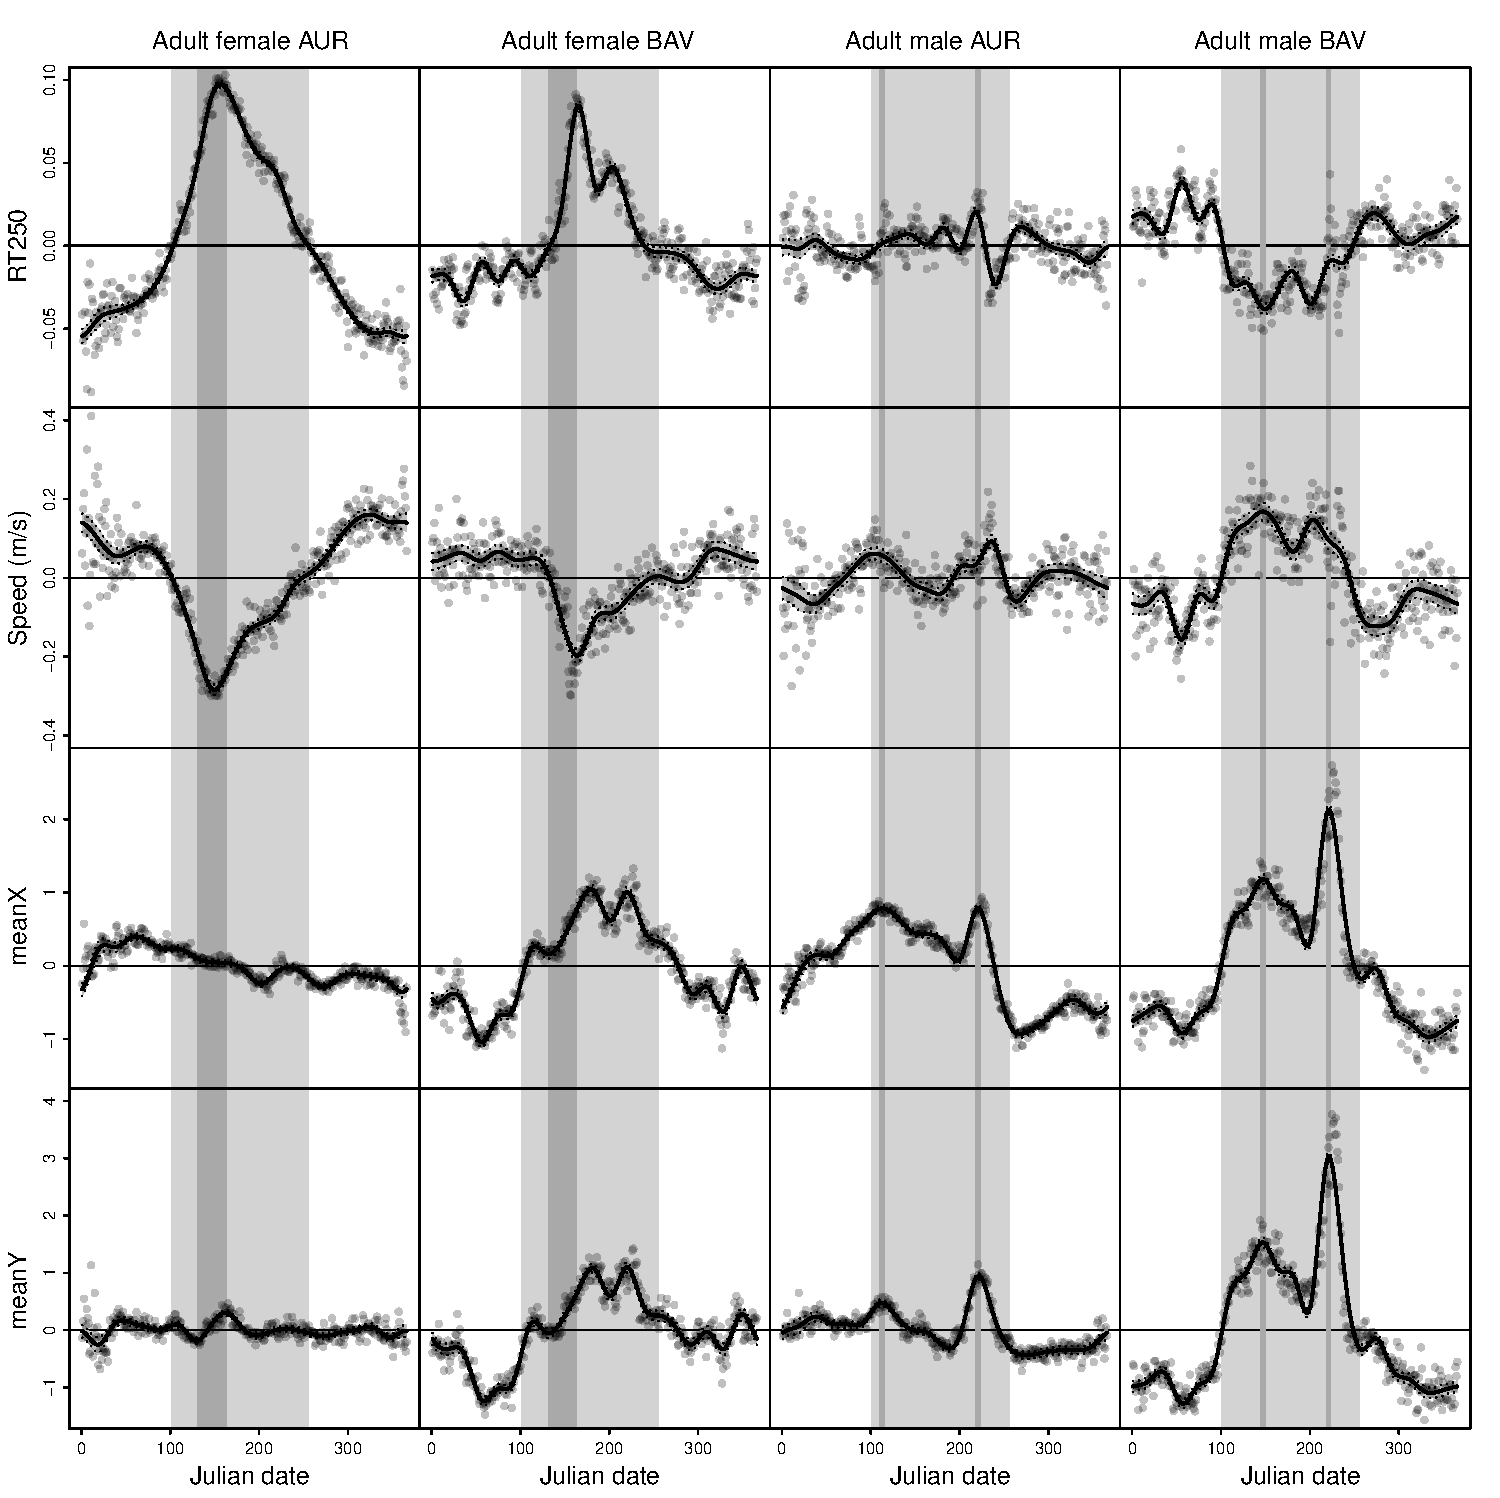
\includegraphics[width=0.9\linewidth]{./figures/Fig2NB.pdf}
  \caption{Temporal variations in residence time within a radius of
    250 m (RT250), movement speed (speed), mean head movements on the
    X axis (meanX) and mean head movements on the Y axis (meanY) for
    adult male and female roe deer in the two study sites (AUR in
    France and BAV in Germany), from 2002 to 2013 in AUR and from 2004
    and 2015 in BAV. The time series starts on the 22nd of
    December. The lines (and dotted lines) represent the separate GAMM
    models for each variable (with the confidence intervals) including
    a smoothed effect of time (Julian date) based on cyclic P-spline,
    which differed among study sites, sexes and age classes. Based on
    the literature, the light gray represents the assumed territorial
    period, from the 1st of April to the 1st of September, and the
    dark gray represents the birth period for females, from the 1st of
    May to the 1st of June. Finally, for males the dark gray lines
    represent the temporal window for the observed peaks in these
    metrics in spring (12th of April and 16th of May for AUR and
    BAV, respectively) and summer (29th of July for AUR and BAV).}\label{fig:sex}
\end{figure}

\newpage
\begin{figure} [!h]
  \centering
  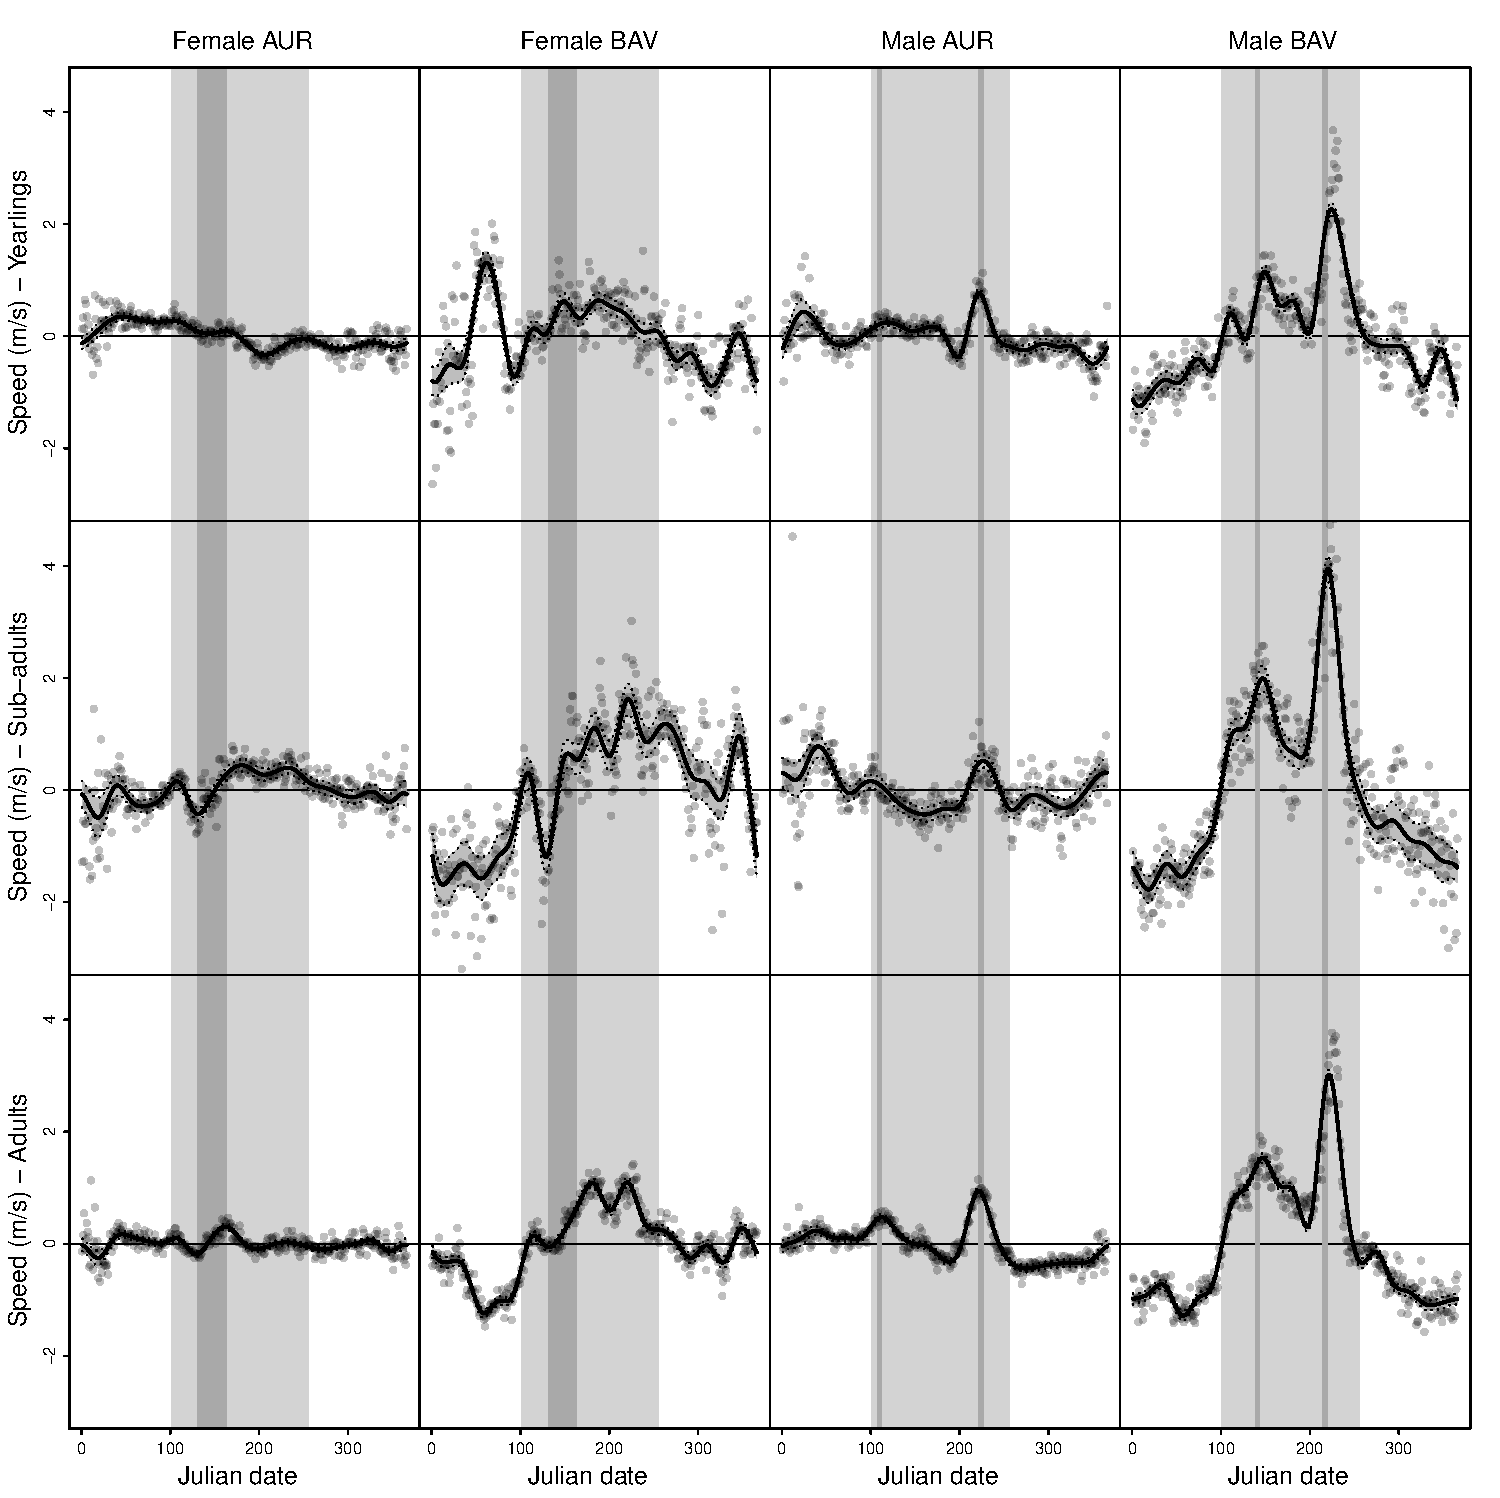
\includegraphics[width=0.9\linewidth]{./figures/Fig3b.pdf}
  \caption{Temporal variations in mean head movements on the Y axis
    for male and female roe deer among age classes in the two study
    sites (AUR in France and BAV in Germany), from 2002 to 2013 in AUR
    and from 2004 and 2015 in BAV. The time series starts on the 22nd
    of December. The lines (and dotted lines) represent the GAMM
    models (with the confidence intervals) including a smoothed effect
    of time (Julian date) based on a cyclic P-spline, which differed
    among study sites, sexes and age classes. Based on the literature,
    the light gray represents the assumed territorial period, from the
    1st of April to the 1st of September, and the dark gray represents
    the birth period for females, from the 1st of May to the 1st of
    June. Finally, for males the dark gray lines represent the
    temporal window for the observed peaks in these metrics in spring
    (12th of April and 16th of May for AUR and BAV, respectively) and 
    summer (29th of July for AUR and BAV).}\label{fig:age}
\end{figure}

\begin{figure} [!h]
  \centering
  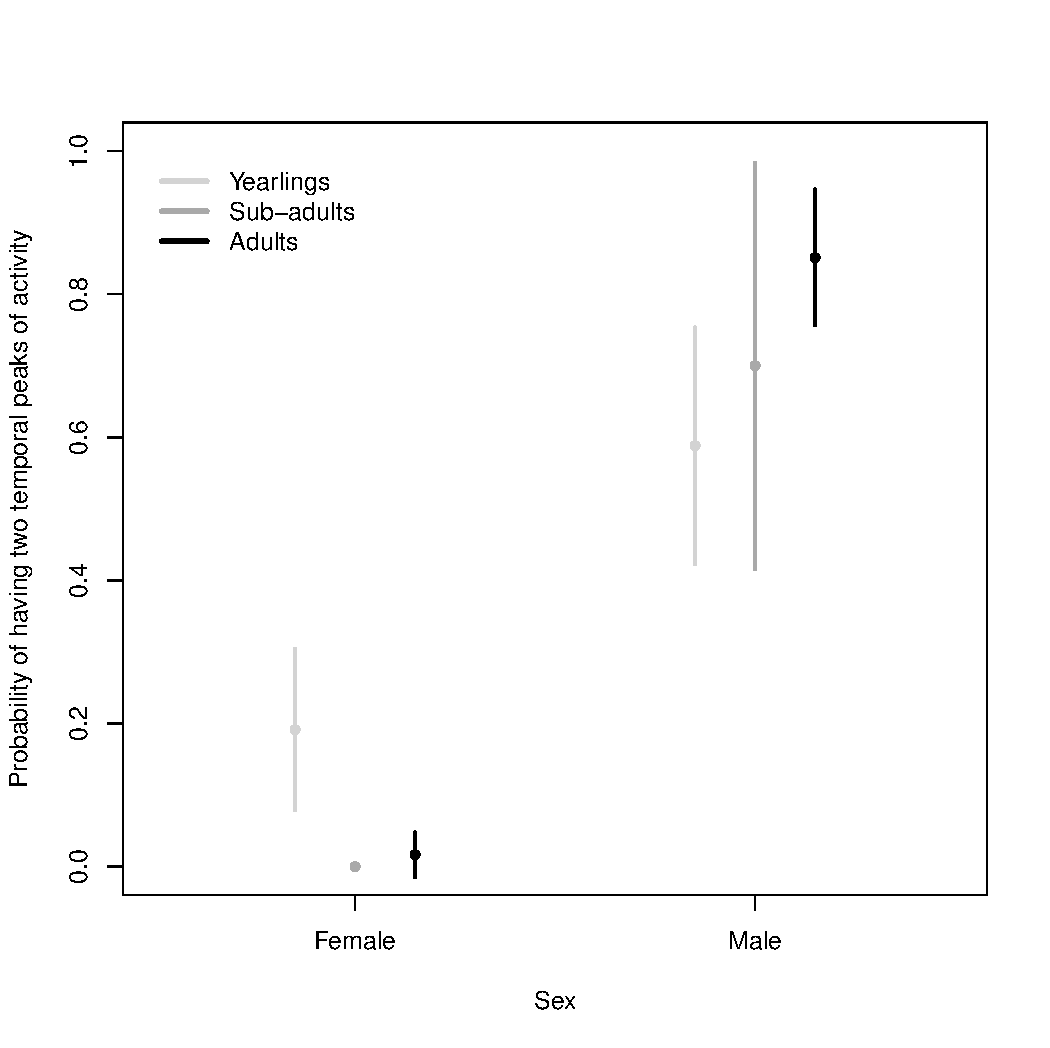
\includegraphics[width=0.5\linewidth]{./figures/Fig4.pdf}
  \caption{The probability of having two temporal peaks of activity in
    relation to the sex and the age class, for roe deer monitored in
    two study sites (AUR in France and BAV in Germany), from 2002 to
    2013 in AUR and from 2004 and 2015 in BAV. The dots (and segment
    lines) represent the GLM models (with the confidence
    intervals).}\label{fig:probability}
\end{figure}

\end{document}
